\section{The patterns of the low-weight PCs}
\label{sec3}
To determine the details of the patterns of the low-weight PCs, we assume $f(x)$ can be factorized into $K$ prime polynomials as 
\begin{align}
f(x)&=\prod_{k=0}^{K-1}f_k^{\gamma_k}(x)
\end{align}
where $\gamma_0,\gamma_1,\cdots,\gamma_{K-1}$ are positive integers and we assume $\varphi_k$ is a root of $f_{k}(x)$ of order $\epsilon_k$.

Refering to \eqref{eq:low-weight-parity}, we consider the solution of
\begin{align}
	h(x) \mod f(x) \equiv 0
	\label{Eq:condition}
\end{align}
%
We start from the simplest case $K=1$, \ie, $f(x) = f_0^{\gamma_0}(x)$. Then, we can see from \eqref{eq:low-weight-parity} that each root is also a root of $h(x)$. For the case $\gamma_0 = 1$, since all $\varphi_0^i$, $0 \leq i < \epsilon_0$, are distinct from each other, the equation
\begin{align}
	h(\varphi_0^i)=0,~~~ 0 \leq i < \epsilon_0
	\label{Eq:rootcondition}
\end{align}
is a necessary and sufficient condition of \eqref{Eq:condition}. 

For $\gamma_0 > 1$, on the other hand, \eqref{Eq:rootcondition} is necessary but not sufficient for \eqref{Eq:condition}. For this case, although we may derive some solutions by differential equations
\begin{align}
\left.\frac{d^{(j)}h(x)}{d x^j}\right|_{x=\varphi_0^i}=0,~~~0 \leq i < \epsilon_0,~1 \leq j < \gamma_0
\label{Eq:differential}
\end{align}
we can not determine the patterns completely, since the operations on coefficients of the polynomial are performed on the terms $\bmod~ p$. Thus, we need to remove possible ghost solutions at further confirmation step.

For the case where $K>1$, we may repeat the above discussion for the roots $\varphi_k$, $0 < k < K$, and take the intersection of the results to determine the low-weight PC patterns.

\subsection{The pattern of the weight-2 PCs}
\label{sec:PC2}
Each weight-2 PC can be written as 
\begin{equation}
h(x)=1+x^{\alpha}
\label{eq:wt2-gen-form}
\end{equation}
without loss of generality. Thus from \eqref{Eq:rootcondition}, we have 
\begin{equation}
(\varphi_0^i)^{\alpha} =1,~~~ 0 \leq i < \epsilon_0
\label{novelEq5b}
\end{equation}
On the other hand, the order of $\varphi_0,~\epsilon_0$ is the least integer satisfying $\varphi_0^{\epsilon_0} \equiv 1$, thus, $\alpha$ should satisfy the condition
\begin{equation}
\alpha \bmod \epsilon_0  \equiv 0 
\label{eq:wt2-alpha}
\end{equation}

\subsection{The pattern of the weight-3 PCs}

Each weight-3 PC can be written as 
\begin{equation}
h(x)=1+x^{\alpha}+x^{\beta},~\alpha < \beta
\label{novelEqwt3}
\end{equation}
without loss of generality. 
Thus, $(\alpha,\beta)$ should satisfy the condition
\begin{equation}
\varphi_0^{\alpha}+\varphi_0^{\beta}= 1
\label{Eq:novelEq5b}
\end{equation}
Such pairs can be found by referring to the table of the extended field for $\GF\left(2^M\right)$. 
Let $(m,n)$ be such a pair, and we let $\cM=\epsilon_0 \ell+m$ and $\cN=\epsilon_0 \ell+n$, $\ell \geq 0$. Then it is obvious that each pair $(\alpha,~\beta) \in \cM \otimes \cN$ satisfies
\eqref{Eq:novelEq5b}. For a fixed $\alpha$, on the other hand, since $\alpha+i$, $0 \leq i < \epsilon_0$, are distinct from each other, any integer $\beta$ that satisfies \eqref{Eq:novelEq5b} must be such that $n\equiv \beta \mod \epsilon_0$.

%Furthermore, let  We denote the set of all pairs as $\cM \bar{\otimes} \cN$, where the elements of this set are formed using a tensor product approach. Then, $(\alpha,~\beta) \in \cM \bar{\otimes} \cN$
\subsection{Examples}

\begin{example}$f(x)=1+x+x^2$

$f(x)$ is a primitive polynomial and since $x^1=x$, $x^2 \equiv 1+x$, and $x^3 \equiv 1 \bmod f(x)$, the order of the root $\varphi_0$ is $\epsilon_0=3$.\newline
\textbf{Weight-2 PCs}: 
 From \eqref{eq:wt2-alpha}, it is obvious that $\alpha$ should be a multiple of $3$. The corresponding values for $a(x)$ and $h(x)$ are shown in Table \ref{novelTab2} for the first four valid values of $\alpha$.
\begin{table}[htbp]
%\parbox{.5\linewidth}{
 \caption{$f(x)=1+x+x^2$}
\centering
 \begin{tabular}{c c c} 
%\hline
 $a(x)$ & $h(x)$ \\ [0.5ex] 
 \hline\hline
$1+x$
 & $1+x^{3}$ \\
\hline
$1+x+x^3+x^4$
 & $1+x^{6}$ 
 \\
\hline
$1+x+x^3+x^4+x^6+x^{7}$ 
&  $1+x^{9}$ 
\\
\hline
$1+x+x^3+x^4+x^6+x^{7}+x^9+x^{10}$
 &  $1+x^{12}$ \\
 \end{tabular}
 \label{novelTab2}
\end{table}
We may write the weight-2 PCs in general form as $h(x)=1+x^{3\ell}$, $\ell>1$, and the corresponding $a(x)$ is given by 
\begin{equation*}
a(x)=\sum_{i=0}^{\ell-1} x^{3i}(1+x)
\end{equation*}

\textbf{Weight-3 PCs}: The elements of GF$(2^2)$ are shown in Table \ref{novelTab7}.  We can see from this table that $(m,n)= (1,2)$ and, consequently, let $\cM = \{3\ell+1\}_{\ell\geq 0}$ and $\cN = \{3\ell+2\}_{\ell\geq 0}$. Then, we have $(\alpha,\beta) \in \cM\otimes\cN$.  

The corresponding values for $a(x)$ and $h(x)$ are shown in Table \ref{novelTab8} below for the first four valid values of $(\alpha,\beta)$ and the weight-3 PCs can be written as $h(x)=1+x^{3\ell_0+1}+x^{3\ell_1+2},~\ell_0,~\ell_1 \geq 0$
in general form. 
 \begin{table}[htbp]
 \caption{Non-zero Elements of $\GF \left(2^2\right)$ generated by $f(x)=1+x+x^2$}
\centering
 \begin{tabular}{c c} 
 \hline
 power representation & polynomial representation \\ [0.5ex] 
 \hline\hline
$x^0~=x^3=1$ & $1$\\
\hline
$x$ & $x$\\
\hline
$x^2$ &  $1+x$\\
\hline
 \end{tabular}
 \label{novelTab7}
\end{table}

\begin{table}[htbp]
 \caption{$f(x)=1+x+x^2$}
\centering
 \begin{tabular}{c c} 
 \hline
 $a(x)$ & $h(x)$\\ [0.5ex] 
 \hline\hline
$1$ & $1+x+x^2$\\ 
\hline
$1+x+x^2$ &  $1+x^2+x^4$\\
\hline
$1+x+x^3$ & $1+x^4+x^5$\\
\hline
$1+x^2+x^3$ & $1+x+x^5$ 
 \end{tabular}
 \label{novelTab8}
\end{table}


\label{ex-1}
\end{example}




\begin{example}
$f(x)=1+x+x^2+x^3+x^4$

For this polynomial, we can confirm the order of $\varphi_0$ is $\epsilon_0=5< 15$. Thus, $f(x)$ is a prime but not primitive polynomial.
\newline
\textbf{Weight-2 PCs}: 
From \eqref{eq:wt2-alpha}, $\alpha$ should be a multiple of $5$. The corresponding values for $a(x)$ and $h(x)$ are shown in Table \ref{novelTab3} with general forms for $\ell>1$

%}
\begin{table}[htbp]
%\parbox{.5\linewidth}{
\caption{$f(x)=1+x+x^2+x^3+x^4$}
\centering
\begin{tabular}{c c} 
 \hline
 $\alpha(x)=\sum_{i=0}^{\ell-1} x^{5i}(1+x)$ & $h(x)=1+x^{5\ell}$  \\ [0.5ex] 
 \hline\hline
$1+x$ &$1+x^5$\\ 
$1+x+x^5+x^6$ &$1+x^{10}$  \\
$1+x+x^5+x^6+x^{10}+x^{11}$ & $1+x^{15}$ \\
$1+x+x^5+x^6+x^{10}+x^{11}+x^{15}+x^{16}$ &$1+x^{20}$  
 \end{tabular}
 \label{novelTab3}
%}ll
\end{table}
\textbf{Weight-3 PCs}:
We refer to Table \ref{novelTabWt3-2} and confirm that there is no pair $(m,~n)$ that satisfies $x^m+x^n \equiv 1$. Thus, there are no weight-3 PCs for $f(x)$
 \begin{table}[htbp]
 \caption{Non-zero Elements of $\GF (2^4)$ generated by $f(x)=1+x+x^2+x^3+x^4$}
\centering
 \begin{tabular}{c c} 
 \hline
 power representation & polynomial representation \\ [0.5ex] 
 \hline\hline
$x^0~=x^5~=x^{10}~=x^{15}$ & $1$\\
\hline
$x~=x^6~=x^{11}$ & $x$\\
\hline
$x^2~=x^7~=x^{12}$ &  $x^2$\\
\hline
$x^3~=x^8~=x^{13}$ &  $x^3$\\
\hline
$x^4~=x^9~=x^{14}$ &  $1+x+x^2+x^3$\\
\hline
 \end{tabular}
 \label{novelTabWt3-2}
\end{table}
\label{ex-2}
\end{example}

\begin{example}
	$f(x)=1+x^2$\newline
	We can write $f(x)$ as
	\[
	f(x)=(1+x)^2\]
	and the order of the root $\varphi_0$ is $\epsilon_0=1$.
	
	\textbf{Weight-2 PCs}: We obtain from \eqref{Eq:rootcondition} and \eqref{Eq:differential}
	\begin{align}
		(\varphi_0)^{\alpha} = 1
		\label{Eq:example31}
	\end{align}
	and
	\begin{align}
		\alpha(\varphi_0)^{(\alpha-1)} = 0
		\label{Eq:example32}
	\end{align}	
	respectively. Although \eqref{Eq:example31} implies $\alpha$ in \eqref{eq:wt2-alpha} can be any positive integer, we can see from \eqref{Eq:example32} that $\alpha$  should be an even number.
	The corresponding values for $a(x)$ and $h(x)$ are shown in Table \ref{novelTab1} with general forms for $\ell>1$.
	\begin{table}[htbp]
		\renewcommand{\arraystretch}{1.3}
		%\parbox{.3\linewidth}{
		\caption{$f(x)=1+x^2$}
		\centering
		\begin{tabular}{c c } 
			\hline
			$\alpha(x)=\sum_{i=0}^{\ell-1} x^{2i}$ & $h(x)=1+x^{2\ell}$ \\ [0.5ex] 
			\hline\hline
			$1$ & $1+x^2$\\ 
			$1+x^2$ & $1+x^4$ \\
			$1+x^2+x^4$ & $1+x^6$\\
			$1+x^2+x^4+x^6$ & $1+x^8$ 
		\end{tabular}
		\label{novelTab1}
	\end{table}
	
	\textbf{Weight-3 PCs}:
	With the same reason of Example \ref{ex-2}, there are no weight-3 PCs associated with $f(x)$.
\label{ex-3}
\end{example}


%=====================Deleted Examples  =======================%
%\begin{example}
%$f(x)=1+x^2+x^3+x^4$\newline
%$f(x)$ can be written as 
%$$f(x)=\prod_{k=0}^{1}f_k(x)$$
%where 
%$$f_0(x)=1+x,~f_1(x)=1+x+x^3$$ 
%For $f_0(x), x \equiv 1$, and $x^1 \equiv 1 \bmod f_0(x)$, which means the order of the root $\varphi_0$ is $\epsilon_0=1$ and $\alpha_0$ should be a multiple of $1$. Again, for  $f_1(x), x^3 \equiv 1+x$, and $x^7 \equiv 1 \bmod f_1(x)$, which means the order of the root $\varphi_1$ is $\epsilon_1=7$ and $\alpha_1$ should be a multiple of $7$.
%Finally, valid values of $\alpha$ should be a multiple of the least common multiples of $\alpha_0$ and $\alpha_1$, which means $\alpha$ should be a multiple of $7$.
%The corresponding values for $a(x)$ and $h(x)$ are shown in Table \ref{novelTab1-a} with general forms for $\ell>1$.
%\begin{table}[htbp]
%\renewcommand{\arraystretch}{1.3}
%\parbox{.3\linewidth}{
 %\caption{$f(x)=1+x^2+x^3+x^4$}
 %\centering
%\begin{tabular}{c c } 
%\hline
 %$\alpha(x)=\sum_{\ell=0}^{L-1} x^{7\ell}(1+x^2+x^3)$ & $h(x)=1+x^{7\ell}$ \\ [0.5ex] 
%\hline\hline
%$1+x^2+x^3$ & $1+x^7$\\ 
%$1+x^2+x^3+x^7+x^9+x^{10}$ & $1+x^{14}$ \\
%$1+x^2+x^3+x^7+x^9+x^{10}+x^{14}+x^{16}+x^{17}$ & $1+x^{21}$
%\end{tabular}
% \label{novelTab1-a}
%\end{table}
%\end{example}

%\begin{example}
%$f(x)=1+x+x^2+x^3+x^4+x^5+x^6$\newline
%$f(x)$ can be written as 
%$$f(x)=\prod_{k=0}^{1}f_k(x)$$
%where 
%$$f_0(x)=1+x^2+x^3,~f_1(x)=1+x+x^3$$ 
%For $f_0(x), x^3 \equiv x^2+1$, and $x^7 \equiv 1 \bmod f_0(x)$, which means the order of the root $\varphi_0$ is $\epsilon_0=7$ and $\alpha_0$ should be a multiple of $7$. Again, for  $f_1(x), x^3 \equiv 1+x$, and $x^7 \equiv 1 \bmod f_1(x)$, which means the order of the root $\varphi_1$ is $\epsilon_1=7$ and $\alpha_1$ should be a multiple of $7$.
%Finally, valid values of $\alpha$ should be a multiple of the least common multiples of $\alpha_0$ and $\alpha_1$, which means $\alpha$ should be a multiple of $7$.
%The corresponding values for $a(x)$ and $h(x)$ are shown in Table \ref{novelTab1-b} with general forms for $\ell>1$.
%\begin{table}[htbp]
%\renewcommand{\arraystretch}{1.3}
%\parbox{.3\linewidth}{
% \caption{$f(x)=1+x+x^2+x^3+x^4+x^5+x^6$}
 %\centering
%\begin{tabular}{c c } 
%\hline
 %$\alpha(x)=\sum_{\ell=0}^{L-1} x^{7\ell}(1+x)$ & $h(x)=1+x^{7\ell}$ \\ [0.5ex] 
%\hline\hline
%$1+x$ & $1+x^7$\\ 
%$1+x+x^7+x^8$ & $1+x^{14}$ \\
%$1+x+x^7+x^8+x^{14}+x^{15}$ & $1+x^{21}$
%\end{tabular}
% \label{novelTab1-b}
%\end{table}
%\end{example}
%=====================================End of deleted examples========================%
\begin{example}
$f(x)=1+x^2+x^3+x^4+x^6$

The given polynomial can be written as 
$$f(x)=\prod_{k=0}^{1}f_k(x)$$
where 
$$f_0(x)=1+x+x^2,~f_1(x)=1+x+x^2+x^3+x^4$$ 
and we know from Example \ref{ex-1} and Example \ref{ex-2} that $\epsilon_0=3$ and $\epsilon_1=5$ respectively.

\textbf{Weight-2 PCs}: 
From \eqref{eq:wt2-alpha} , the valid values of $\alpha$ should be a multiple of $\epsilon_0$ and $\epsilon_1$, hence, $\alpha$ should be a multiple of $\lcm(\epsilon_0,\epsilon_1)=15$.
The corresponding values for $a(x)$ and $h(x)$ are shown in Table \ref{novelTab1-c} with general forms for $\ell>1$.

\begin{table}[htbp]
\renewcommand{\arraystretch}{1.3}
%\parbox{.3\linewidth}{
 \caption{$f(x)=1+x^2+x^3+x^4+x^6$}
 \centering
\begin{tabular}{c c } 
\hline
 $\alpha(x)=\sum_{i=0}^{\ell-1} x^{15i}(1+x^2+x^3+x^6+x^7+x^9)$ & $h(x)=1+x^{15\ell}$ \\ [0.5ex] 
\hline\hline
$1+x^2+x^3+x^6+x^7+x^9$ & $1+x^{15}$\\ 
$1+x^2+x^3+x^6+x^7+x^9+x^{15}+x^{17}+x^{18}+x^{21}+x^{22}+x^{24}$ & $1+x^{30}$ \\
\end{tabular}
 \label{novelTab1-c}
\end{table}

\textbf{Weight-3 PCs}:
Since we have shown in Example \ref{ex-2} that $f_1(x)$ does not yield any weight-3 PC, there are no weight-3 PCs associated with $f(x)$.
%We may write the weight-2 PCs in general form as $h(x)=1+x^{7\ell},~\ell>1$ and the corresponding $a(x)$ is given by 
%\begin{equation*}
%a(x)=\sum_{\ell=0}^{L-1} x^{7\ell}(1+x)
%\end{equation*}
\label{ex-4}
\end{example}

\begin{example}
$f(x)=1+x+x^5$

The polynomial $f(x)$ can be written as 
$$f(x)=\prod_{k=0}^{1}f_k(x)$$
where 
$$f_0(x)=1+x+x^2,~f_1(x)=1+x^2+x^3$$ 
We know from Example \ref{ex-1} that $\epsilon_0=3$ and it can be confirmed that $\epsilon_1=7$.

\textbf{Weight-2 PCs}: 
The valid values of $\alpha$ in \eqref{eq:wt2-alpha} should be a multiple of $\lcm(\epsilon_0,\epsilon_1)=21$.
The corresponding values for $a(x)$ and $h(x)$ are shown in Table \ref{novelTab1-c} with general forms for $\ell>1$.

\begin{table}[htbp]
\renewcommand{\arraystretch}{1.3}
%\parbox{.3\linewidth}{
 \caption{$f(x)=1+x+x^5$}
 \centering
\begin{tabular}{c c } 
\hline
 $\alpha(x)=\sum_{i=0}^{\ell-1} x^{21i}(1+x^2+x^3+x^4+x^6+x^8+x^{4}+x^{6}+x^{8}+x^{11}+x^{12}+x^{16})$ & $h(x)=1+x^{21\ell}$ \\ [0.5ex] 
\hline\hline
$1+x^2+x^3+x^4+x^6+x^8+x^{4}+x^{6}+x^{8}+x^{11}+x^{12}+x^{16}$ & $1+x^{21}$\\ 
\end{tabular}
 \label{novelTab1-c}
\end{table}

\textbf{Weight-3 PCs}:
We rewrite $\cM$ and $\cN$ in Example \ref{ex-1} as $\cM^0$ and $\cN^0$, respectively,
and referring Table \ref{novelTabWt3-5} let
\begin{align}
	\cM_0^1 &:= \{7\ell + 1\}_{\ell \geq 0},~\cN_0^1 := \{7\ell + 5\}_{\ell \geq 0}\cr
	\cM_1^1 &:= \{7\ell + 2\}_{\ell \geq 0},~\cN_1^1 := \{7\ell + 3\}_{\ell \geq 0}\cr
	\cM_2^1 &:= \{7\ell + 4\}_{\ell \geq 0},~\cN_2^1 := \{7\ell + 6\}_{\ell \geq 0}
\end{align}
Then, we have
\[
(\alpha_0,~\beta_0) \in \cM^0\otimes\cN^0 
\]
and
\begin{equation*}
\begin{split}
(\alpha_1,~\beta_1) \in &\bigcup_{i=0}^2 \cM_i^1\otimes\cN_i^1 
\end{split}
\end{equation*}
Therefore, by taking intersection, we have $(\alpha,\beta) \in \left(\cM^0\otimes\cN^0\right)\bigcap\left(\bigcup_{i=0}^2 \cM_i^1\otimes\cN_i^1 \right) $.

\begin{table}[htbp]
 \caption{Non-zero Elements of $\GF (2^3)$ generated by $1+x^2+x^3$}
\centering
 \begin{tabular}{c c} 
 \hline
 power representation & polynomial representation \\ [0.5ex] 
 \hline\hline
$x^0~=x^7$ & $1$\\
\hline
$x$ & $x$\\
\hline
$x^2$ &  $x^2$\\
\hline
$x^3$ &  $1+x^2$\\
\hline
$x^4$ &  $1+x+x^2$\\
\hline
$x^5$ &  $1+x$\\
\hline
$x^6$ &  $x+x^2$\\
\hline
 \end{tabular}
 \label{novelTabWt3-5}
\end{table}

The corresponding values for $a(x)$ and $h(x)$ are shown in Table \ref{novelTab8-b} below for the first three valid values of $(\alpha,\beta)$.
%Also, a visual for $(\alpha,~\beta)$ is shown in Fig. \ref{fig:example5-union}, where the union is in dicated by the pairs connected in  Fig. \ref{fig:example5-union}-(a) and  Fig. \ref{fig:example5-union}-(b).
\begin{table}[htbp]
 \caption{$f(x)=1+x+x^5$}
\centering
 \begin{tabular}{c c} 
 \hline
 $a(x)$ & $h(x)$\\ [0.5ex] 
 \hline\hline
$1$ & $1+x+x^{5}$\\ 
\hline
$1+x+x^5$ &  $1+x^2+x^{10}$\\
\hline
$1+x+x^2+x^3+x^4+x^{6}+x^{8}$ & $1+x^{11}+x^{13}$\\
 \end{tabular}
 \label{novelTab8-b}
\end{table}

%\begin{figure}[h]
%\centering
%		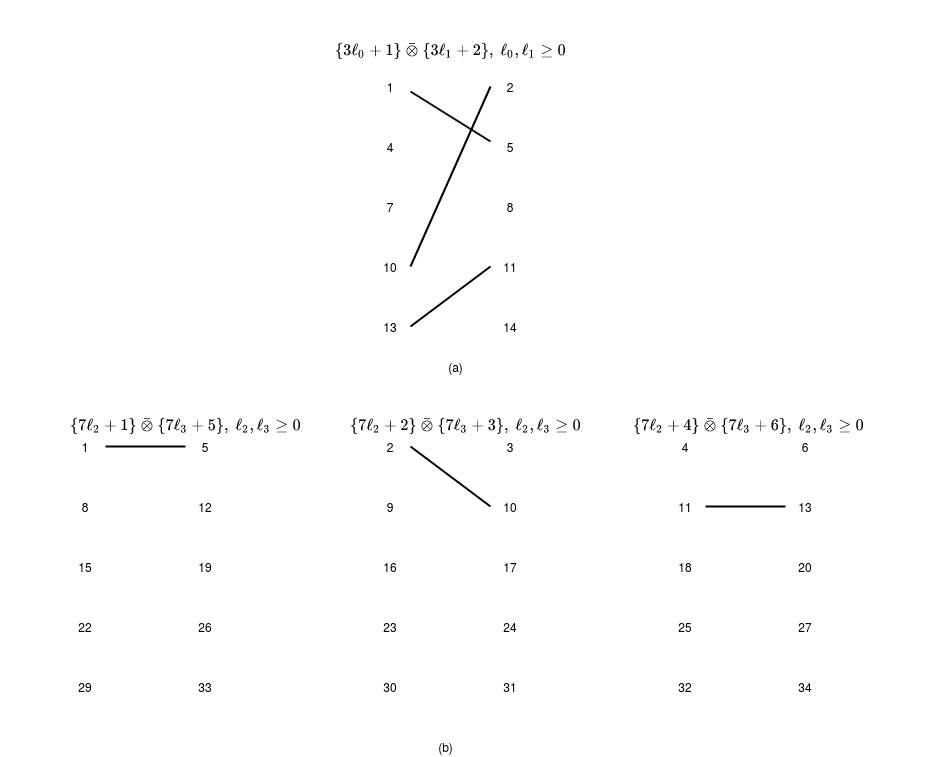
\includegraphics[width=0.45\textwidth]{./ConfSources/pair_union.png}
%		\caption{Visual representation of $(\alpha,~\beta)$ }
%		\label{fig:example5-union}
%		\end{figure}
\label{ex-5}
\end{example}
 







